\documentclass{article}
\usepackage{amsmath}
\usepackage{tikz}
\usepackage{hyperref}
\usetikzlibrary{positioning}
\newcommand\abs[1]{\left|#1\right|}
\newcommand\floor[1]{\lfloor#1\rfloor}

\begin{document}

\title{%
  Introduction to Graph Theory \\
  \large by Richard Trudeau \\
   Ch. 4 Solutions}
   \author{Tyler Bailey}
\maketitle

\begin{enumerate}

	\item[1] $N_1$ is certainly planar, and we proved that it is connected. Prove now that it is polygonal by proving that the statement ``every edge of $N_1$ borders on two different faces" is true.
	
	\textbf{Solution:} This is vacuously true because there are no edges in $N_1$.
	
	\item[2] Omitted. There are many lengthy discussions about fake induction proofs online.
	
	\item[3] Believe it or not, the graph of Figure 104a is planar. Find its number of faces.
	
	\textbf{Solution}: $v = 9$, $e = 20$, so $v + f - e = 2 \implies f = 13$
	
	\item[4] Imitate the proof of Corollary 12 to construct a proof that the graph in 104b is nonplanar.
	
	\textbf{Solution}: Suppose it is planar. By inspection, the figure is not a supergraph of $K_3$, so by Theorem 12, we have $e \leq 2v - 4$. But, inspecting the graph, we see that $v = 8$ and $e = 16$ which implies $16 \leq 12$, a contradiction. Therefore, it must not be planar.
	
	\item[5] Find a polygonal graph G having a face bordering the infinite face which, if removed, results in a subgraph H which is not polygonal.
	
	\textbf{Solution}: Removing the face determined by $(2, 3, 5, 4)$ below would leave us with a graph that is not polygonal, since it would be disconnected.
	
	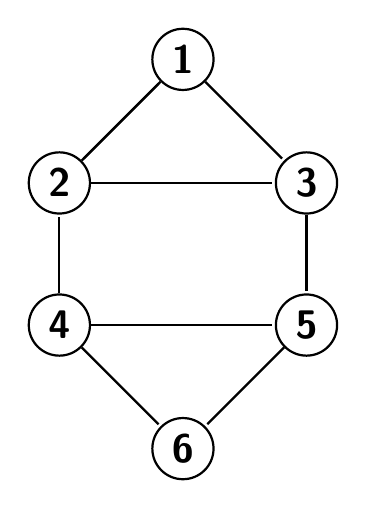
\begin{tikzpicture}[shorten >=1pt,auto,node distance=3cm, thick,main node/.style={circle,draw,font=\sffamily\Large\bfseries}]
			\node[main node] (1) {1};
			\node[main node] (2) [below left=1cm and 1cm of 1] {2};
			\node[main node] (3) [below right=1cm and 1cm of 1] {3};
			\node[main node] (4) [below=1cm of 2] {4};
			\node[main node] (5) [below=1cm of 3] {5};
			\node[main node] (6) [below right=1cm and 1cm of 4] {6};
			\path[every node/.style={font=\sffamily\small}]
				(1)	edge node [left] {} (2)
					edge node [left] {} (3)
                	(2)	edge node [right] {} (3)
                		edge node [right] {} (1)
				(3)	edge node [right] {} (5)
                	(4)	edge node [right] {} (2)
                		edge node [right] {} (5)
					edge node [right] {} (6)
				(5)	edge node [right] {} (6);
		\end{tikzpicture}
	
	\item[6] Prove this partial converse to Euler's formula: If a graph is planar and $v + f - e = 2$, then the graph is connected.
	
	\textbf{Solution}: Suppose the graph is not connected but is planar. Then we can apply Euler's formula to both pieces and get $v_1 + f_1 - e_1 = 2$ and $v_2 + f_2 - e_2 = 2$. Notice that $v = v_1 + v_2$ and $e = e_1 + e_2$ and $f + 1= f_1 + f_2$ (because we double-counted the infinite face). Therefore, we get $v + f - e = v_1 + f_1 - e_1 + v_2 + f_2 - e_2 + 1 = 4 \implies v + f - e = 3$. But, this is a contradiction by Euler's formula, so the graph must have been connected.
	
	\item[7] Let `p' denote the number of components of a graph and prove this generalization of Euler's formula: if a graph is planar, then $v + f - e = 1 + p$.
	
	\textbf{Solution}: We proceed by induction on $p$. We already know that the case $p = 1$ is true because that is just the familiar Euler's formula. Suppose for a graph with $n$ components we have $v + f - e = 1 + n$. Now, given any graph $G$ with $n + 1$ components we can reduce this to a graph $H$ with $n$ components by adding an edge connecting one component to another, which would not change the number of vertices or faces. Therefore, we have $v_H + f_H - e_H = 1 + (n + 1) \iff v_H + f_H - (e_G + 1) = 1 + (n + 1) \iff v_G + f_G - e_G = 1 + n$, which completes the inductive step to complete the proof.
	
	\textbf{Alternative Solution}: We could instead treat each component as its own graph and apply Euler's formula to each piece. Suppose we have $n$ components. Then we have $\sum_{i}{v_i} + \sum_{i}{f_i} + \sum_{i}{e_i} = 2$. Summing over all $n$ components we have $V + \sum_{i}{f_i} - E = 2n$ but doing it this way we accidentally counted the infinite face $n$ times in total, so we should have $V + \sum_{i}{f_i} - E - (n - 1) = 2n \implies V + F - E = 1 + n$

	\item[8] Use corollary 13 to show the graph in Figure 106 is nonplanar:
	
	\textbf{Solution}: Every vertex has degree 6, so by corollary 13, it cannot be planar.
	
	\item[9] Omitted, see the answer in the book.
	
	\item[10] Prove: Every planar graph with $v \geq 4$ has at least $\it{four}$ vertices of degree $\leq 5$.
	
	\textbf{Solution}: Suppose not. And suppose $G$ is ``almost planar" in the sense that if we add a single new edge between any two nodes then the graph will be nonplanar (Note: we can always derive such a graph from planar graphs via connecting successive edges). Now, there can be no vertices with degrees 0 or 1 (if there were, we should connect them to another vertex in the face they are in). And, there are no vertices of degree 2. If there was a vertex of degree 2, then there would be a face of length 4 or more where we could connect it via an edge. So, every vertex has degree $\geq 3$. Suppose $G$ has at most 3 vertices of degree $< 5$. Then $2e \geq 6(v - 3) + 3 \cdot 3 = 6v - 9$. But, we know $e \leq 3v - 6 \implies 2e \leq 6v - 12$. From those two inequalities we derive a contradiction.
	
	\item[11] Find the connectivity $c$ of each graph in Figure 91, 92, 93.
	
	\textbf{Solution}: Respectively: $c = 2, 2, 3, 1, 3, 2$
	
	\item[12] By Exercise 11 of Chapter 2, $2e/v$ is the average of the degrees of a graph. Prove that if a graph has connectivity $c$ then $c \leq 2e/v$.
	
	\textbf{Solution}: Suppose $c > 2e/v$.
	\begin{align}
		c > 2e/v 
		&\iff cv > 2e = \sum_{v} \mathrm{deg}(v) \\
		&\iff \sum_{v} c > \sum_{v} \mathrm{deg}(v)\\
		&\iff c > \mathrm{deg}(v)
	\end{align}
	for some $v$.
	
	But then if we remove the $\mathrm{deg}(v)$ vertices connected to $v$, $G$ will be disconnected because $v$ is isolated. That means that $c$ was not the connection because it was not the minimum such value to disconnect the graph $G$.
	
	\item[13] Use the previous exercise to show that there is no graph with $e = 7$ and $c = 3$, and none with $e = 11$ and $c = 4$.
	
	\textbf{Solution}:
		\begin{enumerate}
			\item[a] Since $e = 7$, we must have $v \geq 5$ (using the fact that $v_{K_4} = 6$). Then, $c \leq 2e/v \implies 3 \leq \floor{14/5} = 2$, a contradiction.
			\item[b] Since $e = 11$, we must have $v \geq 6$ (using the fact that $v_{K_5} = 10$). Then, $c \leq 2e/v \implies 4 \leq \floor{22/6} = 3$, a contradiction.
		\end{enumerate}
	
	\item[14] In a planar graph a bridge necessarily borders on only one face, and an edge bordering on only one face is necessarily a bridge. Thus bridges are the things that prevent planar connected graphs from being polygonal. Use this fact to prove that if a planar and connected graph $G$ has the property that the boundary of every face is a cyclic graph, then $G$ is polygonal. Then show that the converse statement is false by finding a polygonal graph having a face whose boundary is not a cyclic graph.
	
	\textbf{Solution}:
	
	Counterexample: From problem 1, $N_1$ is polygonal. But, cyclic graphs are only defined when $v \geq 3$, so $N_1$ is not cyclic.
\end{enumerate}

\end{document}